% !TEX root =  ../main.tex
\section{Spread}

\subsection{Definition}

\subsubsection{Signature} \cstr{spread(s : set<VM>)}

\begin{itemize}
\item \cstr{s} : a set of at least 2 VMs for a meaningful constraint. VMs not in the \st{Running} state are ignored.
\end{itemize}

The \cstr{spread} constraint forces all the running VMs in \cstr{s} to be hosted
on distinct servers at any time, even during the reconfiguration process.

\classification{spread}{application administrator}{VM placement,Actions schedule}{Fault tolerance,VM-to-VM placement,Partitioning}

\subsubsection{Usage}

The \cstr{spread} constraint may be used by an application administrator to provide to a replicated service,
fault tolerance to hardware failures. By hosting each replicas on a distinct server, the service will  be
available while at least one server is still online. To achieve this purpose, one \cstr{spread} constraint can
be used with the replicas provided as arguments.


\subsubsection{Example}

Figure~\ref{fig: spread} depicts a sample reconfiguration between a source and a destination
configuration. In this example, the following \cstr{spread} constraints were considered:

\begin{reconfiguration}
\centering
\begin{minipage}[b]{0.40\textwidth}
\begin{lstlisting}
N1: VM1 VM2
N2: VM3 VM4 VM5
N3: VM6
\end{lstlisting}
\end{minipage}
\begin{minipage}[b]{2cm}
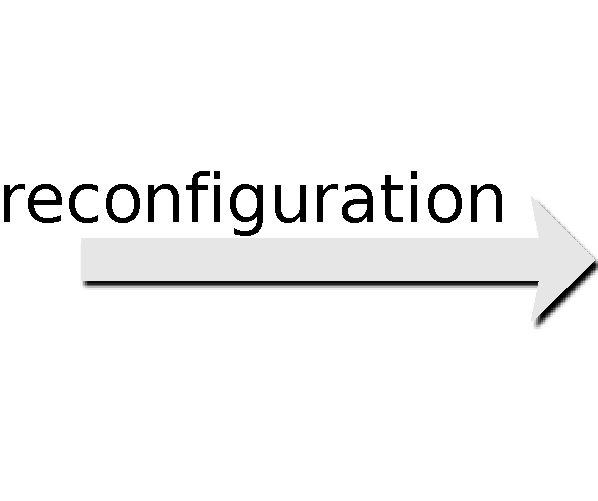
\includegraphics[width=2cm]{img/arrow_reconfiguration}
\end{minipage}
\begin{minipage}[b]{0.40\textwidth}
\begin{lstlisting}
N1: VM1 VM6
N2: VM3 (VM4)
N3: VM2 VM5
\end{lstlisting}
\end{minipage}
\caption{A reconfiguration motivated by \cstr{spread} constraints.}\label{fig: spread}
\end{reconfiguration}

\begin{itemize}

\item \cstr{spread(\{VM1,VM2\})}. This constraint was not satisfied in the source configuration as both VMs were colocated.
%
The reconfiguration fixed this violation by relocating \cstr{VM2} to \cstr{N3}.

\item \cstr{spread(\{VM3, VM4\})}. This constraint was not satisfied in the source configuration.
Putting \cstr{VM4} in the \st{Suspended} state fixed this violation without having to perform a relocation.

\item \cstr{spread(\{VM5, VM6\}}). This constraint was satisfied in the source configuration. However, let consider
\cstr{VM5} must be running on \cstr{N3}, which was already hosting \cstr{VM6}. In this setting, \cstr{VM6}
has been relocated to \cstr{N1} to disallow the colocation. Furthermore, to prevent from a temporary colocation on \cstr{N3}, it was a necessary to relocate \cstr{VM6} before \cstr{VM5}. Figure~\ref{fig: spread plan} depicts the associated event-based reconfiguration plan.
\end{itemize}


\begin{reconfPlan}[htb]
\centering
\begin{tabular}{ll}
\O & $\rightarrow$ stop(VM4) \& relocate(VM5)\\
!relocate(VM5)\ & $\rightarrow$ relocate(VM6)\\
!relocate(VM6)\ & $\rightarrow$ relocate(VM2)
\end{tabular}
\caption{Event-based reconfiguration plan associated to the reconfiguration depicted in Figure~\ref{fig: spread}.}\label{fig: spread plan}
\end{reconfPlan}

\fullVersion{
\subsection{Model}

The \cstr{spread} constraint is modeled using negations between the d-slice placement variables of the running VMs to ensure all the running VMs will be hosted on distinct servers by the end of the reconfiguration process.
To prevent from a temporary overlap during the reconfiguration process, precedence relations between the slices are established. When a d-slice associated to a VM has to be hosted on a server that is currently hosting another (but necessarily leaving) involved VM, then the relocation is delayed until the VM has leaved the server.

\begin{equation*}
\begin{split}
\text{\cstr{spread}}&\text{\cstr{(V : set<VM>)}} \triangleq\\
   & \forall v_i,v_j \in V,\\
   & d_i^h \neq d_j^h \wedge\\
   & d_i^{h} = c_j^{h} \Rightarrow d_i^{st} \geq c_j^{ed}
\end{split}
\end{equation*}

\subsection{Availability}

\subsubsection{In {\btrp}} 
This constraint is available in {\btrp} using the name \texttt{Spread}.
Using the global constraint catalog, the assigned for each of the d-slice placement variable is
ensured to be unique  using one \emph{allDifferent}~\cite{allDiff} global constraint.
The non-overlapping of VMs during the reconfiguration process is expressed by establishing an implication between constraints. \emph{Implies} constraints are used to indicate that when
the placement variable of a d-slice equals the placement of the
c-slice of any other involved
VMs  then the arrival time of the d-slice must be greater than or equal to the departure time of the
c-slice.


\begin{equation*}
\begin{split}
\text{\cstr{spread}}&\text{\cstr{(V : set<VM>)}} \triangleq\\
   & \text{\em allDifferent}(\{\forall d_i^h | v_i \in V\}) \\
   & implies(eq(d_i^h, c_i^h), geq(d_i^{st}, c_j^{ed})), \forall v_i, v_j \in V
\end{split}
\end{equation*}

\subsection{Violation Detection}

The detection of the violating elements in \cstr{spread} consists in identifying running VMs that are hosted on a same server. When a server hosts multiple VMs that are involved in a same \cstr{spread} constraint, it is ensured that at least one VM is misplaced. Such a violation detection is however not guarantee to be optimal as it is not possible to know exactly which of the colocated VMs are supposed to be hosted elsewhere. An approximation consists then to select all the colocated VMs.
}

\subsection{See also}

\subsubsection{Related Constraints}
\begin{itemize}
\item \cstrref{gather}: the opposite constraint of \cstr{spread}.
\item \cstrref{lazySpread}: a constraint similar to \cstr{spread} that does not guarantee the non-overlapping of the VMs during the reconfiguration process.
\item \cstrref{split}: a constraint to ensure two sets of VMs do not share servers.

\end{itemize}

\printListOfInheritance{spread}